\chapter{Design}
\label{chapter:design}

This chapter discusses design decisions and justifications of the vehicular priority model and developed Priority Based Traffic Control (PBTC) system. The outcomes discussed in this chapter include the design of an appropriate microscopic model of individual vehicle priority, and design of a new phase control algorithm based on the microscopic vehicle priority model for the PBTC system, to be operated on a two-phase intersection. 

\section{Priority Modeling}

Representative modeling of the priority of vehicles and passengers approaching an intersection is required to effectively design, develop and evaluate the PBTC system within a realistic setting. The model is designed such that the priority of an individual vehicle is proportional to the cost, measured in cents, of stopping and/or delaying the vehicle at a controlled intersection. These dimensions were chosen to represent the priority of a vehicle because they are easily described as a quantitative economic cost. 

A single cost figure is calculated by an aggregation of the current effective delay cost, potential stopping cost, and potential delay cost for each vehicle. The operational stopping cost calculation is designed to model the costs imposed by the mechanical operation of a vehicle when required to stop at a controlled intersection and is based on the velocity, acceleration, mass, and engine efficiency of a vehicle. The delay cost calculation is designed as a measure of the costs incurred by road users that are forced to wait due to congestion or signal controls at an intersection and is is based upon the class of vehicle, an individual notion of urgency, and the number of passenger occupants.

Emphasis has been placed on approximations of cost components that can be calculated efficiently in real-time by a traffic light controller. In order to develop simplified approximations of cost components, the following assumptions have been made about the physical characteristics of vehicles and driver behaviours:

% list of the high level assumptions here 
\begin{itemize}
\item Vehicles are classed as light or heavy, with petrol and diesel engines respectively.
\item Vehicle mass, engine efficiency, and aerodynamic properties are considered constant per vehicle class. Table \ref{vehicleclassconstants} shows a list of constants representing the physic	al properties of each vehicle class.
\item The price per litre for petrol fuel is \$2.24, and diesel fuel \$1.65 (New Zealand Dollars), based upon market values at the time of writing.
\item Hybrid and electric vehicles are not included in the scope of this model and require more sophisticated models for cost estimates that include consideration of systems that affect the stopping or delay cost of these vehicles, such as regenerative braking.
\item Fuel use during idle periods is assumed to be zero by this model as the idle cost for a small number of stops is low and only one stop is typically required for each vehicle in simulation.
\end{itemize}

\begin{table}[H]
\centering
\renewcommand{\arraystretch}{1.25}
 	
	\begin{tabular}{@{}lrr@{}} \toprule
		Quantity & value for light vehicles & value for heavy vehicles \\ \midrule
		Mass & 1,500kg & 15,000kg \\
		Engine efficiency factor & 0.3 & 0.4 \\
		Fuel type & petrol & diesel \\
		Fuel price & \$2.24\text{/}\ell & \$1.65\text{/}\ell \\
		Fuel energy density & 36x10^6 \text{J/}\ell & 36x10^6 \text{J/}\ell \\ \bottomrule
	\end{tabular}
	
	\caption{ Physical vehicle constants per vehicle class used as parameters for the physics based consumption model \cite{kesting2013traffic}. Light vehicles are cars only, heavy vehicles can be buses or trucks within the PBTC system. }
	\label{vehicleclassconstants}
\end{table}

% subsections discussing the design of each measure here:

\subsection{Operational Stopping Cost}

The operational stopping cost of an individual vehicle is the economic cost expended whenever the vehicle is delayed or forced to stop at a controlled intersection. The stopping cost of a vehicle is proportional to the square of the cruise speed of the vehicle before the stop, and recognises that a vehicle that has been forced to stop expends a certain amount of fuel after starting in order to reach the same speed of travel before stopping. Calculating an estimate for the cost of stopping a vehicle involves estimating the number of litres of fuel consumed when decelerating and accelerating at a controlled intersection.

Physics-based consumption models can be used for calculating instantaneous fuel consumption as a function of driving resistance \cite{kesting2013traffic}. An instantaneous fuel consumption model was originally used in simulation as part of a priority message from a vehicle upstream of a traffic signal controller, however it was found that the fuel consumption rate alone is not appropriate for estimating the operational stopping cost of a vehicle, as it is dependent on vehicle speed and acceleration at the instant of communication.

Models exist for retrospective analysis of fuel consumption over a journey, using measured speed and acceleration rates over time and can be used to find the total cost of a stopping and accelerating through a controlled intersection after a vehicle has completed a trip \cite{kesting2013traffic,akcelik2003fuel,trieber2008congestion}. Attempts to implement these models at various time steps to estimate consumption leaving an intersection were not successful at producing meaningful results as an assumed arbitrary rate of predicted acceleration is not appropriate for all vehicles and speed limits. In practice, driver behaviour, vehicle characteristics, and intersection geometries are likely to significantly de crease the accuracy of a predictive acceleration estimation \cite{kesting2013traffic}.

An alternative appropriate measure of operational stopping cost is achieved by the PBTC system through a physics-based consumption model considering the deceleration and acceleration stages of a stop for a particular vehicle. The PBTC system estimates the fuel consumption of a vehicle departing an intersection by calculating the kinetic energy of the vehicle before the stop. By making an assumption that a vehicle will accelerate to their previous approach speed when leaving the intersection, the calculation is a reflection of how much energy is lost if the vehicle is requested to stop as it will require the same amount of energy to reach approach speed. As most modern car engines employ a fuel cutoff mechanism during deceleration to prevent unnecessary fuel use, the total energy used can be approximated solely on the acceleration component of a stop at an intersection. This assumption does not hold in all circumstances, for example whenever downstream links of an intersection are heavily saturated with slow moving traffic, however it is a reasonable estimation for free flowing traffic as the approach and departure speeds are likely to be equal to the speed limit of the area. 

Given the velocity and mass of an approaching vehicle is known, the litres of fuel required to generate this energy can be found based on the calorimetric energy density of the fuel being burned by the engine and the mechanical efficiency factor of the vehicle engine. Equation \ref{fuelconsump} summarises the calculation of the operational stopping cost based on this method.

% equation here
\begin{align}
	\centering
		c_\text{s} = {\frac{\frac{1}{2}m{v}^{2} }{\gamma \times w_\text{cal}}} \times {p_{\text{f/}\ell}}
	\label{fuelconsump}
\end{align}

Where $c_\text{s}$ is the estimated cost of stopping a given vehicle, $m$ and $v$ are the mass and velocity of the vehicle respectively, $\gamma$ is the engine efficiency coefficient for the vehicle engine (typically between 0.25-0.35 for passenger cars), $w_\text{cal}$ is the calorimetric energy density of the engine's fuel, and $p_{\text{f/}\ell}$ is the price per litre of fuel that is being burned by the vehicle's engine.

This physics based consumption model is only an approximation of the actual fuel consumption of approaching vehicles, but appropriately differentiates between light and heavy vehicles. More sophisticated estimations of fuel consumption would be desirable in practice and could be achieved through physics based models, or online learning of accurate measures of fuel consumption. Improving the fuel consumption model described here is recommended as an area of future work. 

\subsection{Delay Cost}
\label{sec:design_delay_cost}

The delay cost of a vehicle approaching a traffic light is dependent on the urgency of travel of the vehicle occupants. Delay costs for a vehicle occupant can be defined proportional to the time available for a passenger to reach a given destination by a predetermined time. For example, consider a passenger is travelling from the Wellington Central Business District (CBD) to the airport and has only ten minutes available before check-in closes for a flight, the cost of delay for the journey should be significantly higher than that of a single occupant vehicle returning to a residence with no urgency of travel. 

The calculation of a delay cost for each vehicle requires user input of the urgency of travel for a passenger or passengers. This project assumes vehicles on the road network are equipped with a dashboard computer capable of receiving user input for any of the required variables. A number of alternative variables of user input have been considered during development of the PBTC system, including arrival time and relative urgency. 

In an arrival time based approach, a user is required to set their destination and desired time of arrival into the dashboard computer, to be sent to a PBTC traffic controller when approaching an intersection. The PBTC controller can estimate the travel time to the destination and based on the arrival time, assign a cost of delay to the vehicle. One of the advantages of this method is that a sophisticated network of connected PBTC controllers could share knowledge of traffic conditions at each intersection and calculate an accurate measure of the likely travel time based on a route to the destination. This approach is disadvantaged by the complexity of user input. For example, if a user does not know the travel time to a destination from their current location, they may inadvertently allocate themselves maximum urgency by setting a short time of arrival and as a result it is more difficult for the system to consider a range of vehicle urgencies.

As an alternative, a relative urgency measure is used by the PBTC system, which requires a driver to set their own perceived urgency as a discrete numerical value on a scale from one to five. This measure is both easy for vehicle occupants to understand, and simple for a PBTC controller to consider relative to other vehicles at an intersection. Passengers can use their knowledge of the approximate travel time to a destination and importance of the journey to make their own judgement about urgency of passage at an intersection. A potential drawback of this system is the ease of which it can be abused, for example all drivers can easily set their urgency to the maximum value. For the purposes of this project, urgency values are assumed to be set honestly by drivers.

For simplicity, the PBTC system assumes that all passengers in a vehicle have identical urgency and as a result, the  delay cost is linearly proportional to the number of passengers in a vehicle. Consequently, vehicles with higher passenger occupancy are favoured by the PBTC system, encouraging more efficient use of road networks through ride-sharing or carpooling initiatives. Reducing the number of single occupant vehicles on roads reduces congestion and fuel emissions and is similarly encouraged by existing initiatives such as High Occupancy Vehicle (HOV) lanes in use on some modern highways with congestion problems \cite{fielding1993hov}.

The economic cost of delay to the vehicle occupants is calculated using an NZTA estimate of \$26.20NZD hour of delay time \cite{wallis2013costs}. The PBTC system makes the assumption that this figure is representative of the cost of delay for an average journey, and hence reflects a single-occupant vehicle with a relative urgency of 3. Assuming $t$ as the time a vehicle is delayed in seconds, $u$ as the discrete relative urgency input by the vehicle occupant/s, and $p$ as the number of passengers in a vehicle, a formula for the overall cost of delaying a vehicle, $c_\text{d}$, is given as

% equation here
\begin{equation}
	c_\text{d} &= t ^{s(u)} \times 0.007(\frac{u}{3}) \times p 
	\label{delaycostequation}
\end{equation}

Where 0.007 is the constant delay cost in cents per second, and $s(u)$ is a function of the vehicle urgency, determined by
% equation here
\begin{equation}
	s(u) = \left\{
	      \begin{array}{lr}
	     	1 & : u \leq 3\\
	         1.1  & : u = 4 \\
	         1.25 & : u = 5
	     \end{array}
	   \right.
	\label{delayslopeequation}
\end{equation}

Figure \ref{delaycosturgency} shows the relationship between delay cost and time delayed for each of the five discrete urgency values for up to sixty seconds of delay. The PBTC system assumes all urgency values are constant and do not change during the time a vehicle is waiting at an intersection, although in a real-world system this model is likely to be too simplistic. Modeling additional cases was not determined to be relevant within the simulation environment. 

%Depending on the initial urgency of the vehicle, as the length of time that vehicle has been delayed increases, their urgency to pass the intersection will also increase and the costs of delay will compound. There is also a limit to this relationship, for example, if the occupants of a vehicle are delayed to the point that they miss their meeting, flight, or other appointment, their urgency may reduce significantly and/or they may change destination and return home.

\begin{figure}[]
\centering
	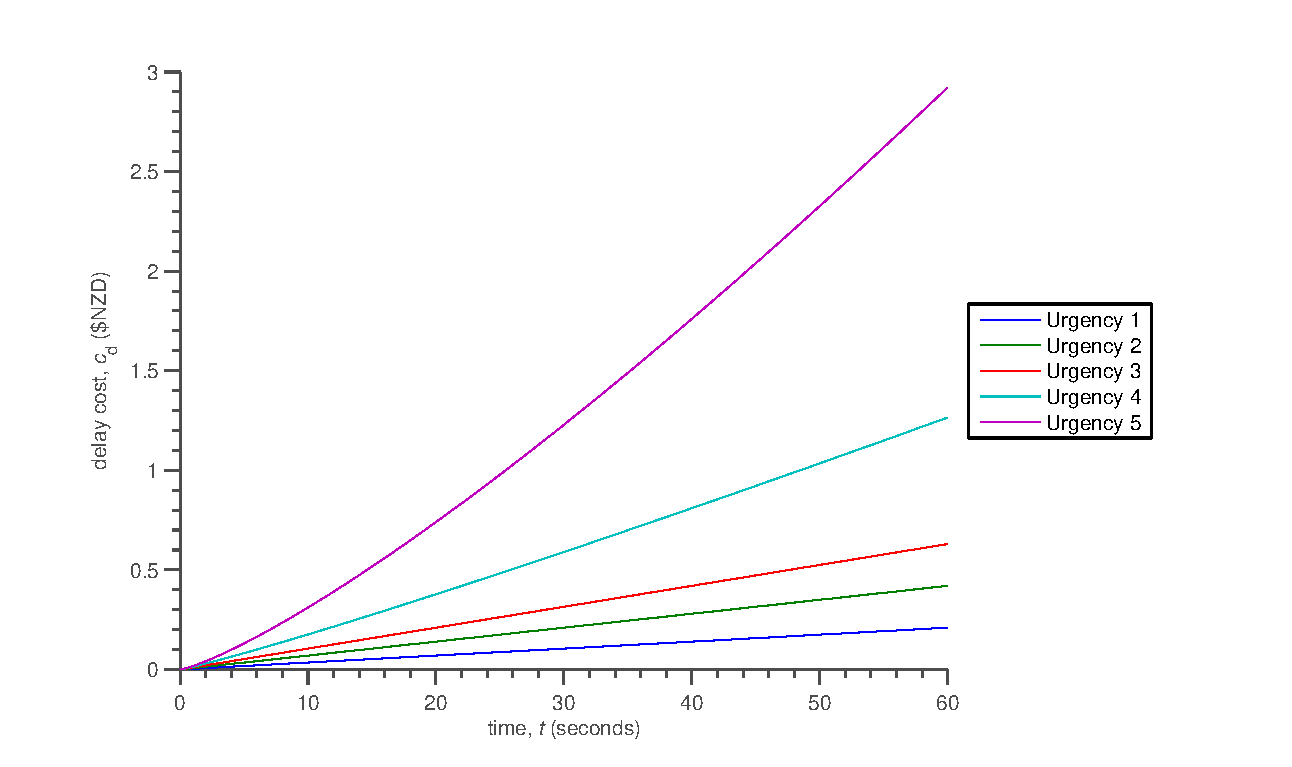
\includegraphics[scale=0.65]{delay_cost_per_urgency.eps}
	\caption{Relationship between cost of delay and time for each passenger urgency value, for up to sixty seconds. }
\label{delaycosturgency}
\end{figure}

\section{PBTC System Design}
 
As no explicit information is available with respect to the cost of stopping and delay for vehicles approaching a given intersection, modern traffic control algorithms typically attempt to reduce delay time or degree of intersection saturation in the hope of reducing congestion and improving the quality of travel. To reduce the costs of travel incurred by vehicles approaching a controlled intersection, the PBTC system is required to consider the costs of delay and stopping for approaching vehicles when making signal switching decisions.

\subsection{Assumptions}

Design of a system for producing an optimal, minimal cost solution to phase assignment at any arbitrary controlled intersection is a difficult problem and evaluating such a system requires a sophisticated simulator capable of realistically modeling real world intersection geometrics, driver behaviours, and traffic flows. Development of all of these capabilities for simulation is an effort beyond the scope of this project. For this reason, the following assumptions have been made to simplify development of the PBTC control algorithm within this project:

\begin{itemize}
\item the control algorithm operates over a two-phase intersection, with each phase allocating green to one of two flows of traffic approaching the intersection only,
\item approaching vehicles represent straight through demand for the intersection only, no left/right split phases (i.e ``arrow lights") are required,
\item the algorithm is limited to a single, isolated intersection and does not consider any aspects of coordination between neighbouring intersection controllers.
\end{itemize}

\subsection{Vehicle-Controller Communication}

Communication between vehicles and a PBTC controller at an intersection is required to provide inputs to the control algorithm to determine a cost effective allocation of phase timings based on the real-time traffic conditions. Appendix \ref{appendix:inter-vehicle-comms} outlines the current state of research related to vehicle communication networks. The design and implementation details of the required communication network is not included in the scope of this project and suggested as an area for future research. This project assumes that all of the necessary technology required for vehicles to send small packets of information to a controller exists in every vehicle using a road network, and each vehicle sends its own state information directly to a roadside intersection controller every 2 seconds, within a range of 150 metres.

The 150 metre broadcast window is designed to allow the PBTC controller to be able to respond to approaching vehicles before they reach the intersection stop-line and avoid stopping vehicles if it is unnecessary. Consider a situation where a single vehicle is approaching a red light at an intersection where there is no demand for the competing green phase; in a stop-line actuated control system the vehicle will be forced to stop, wait at least six seconds for the lights to react and change phase, and then take off \cite{scatstraining}. In the PBTC system, the controller can respond to the vehicle demand without requiring the vehicle to stop. The 150 metre window is based on assuming an approaching vehicle is traveling at a constant speed below 80km/h (approximately 22 m/s), requiring at least 133 metres of clearance given a typical controller requires six seconds of intergreen time to change a phase. In practice, it might be useful to be able to adjust the distance at which cars would be considered by the PBTC system based on the speed limit of the area. 

\begin{figure}[]
\centering
	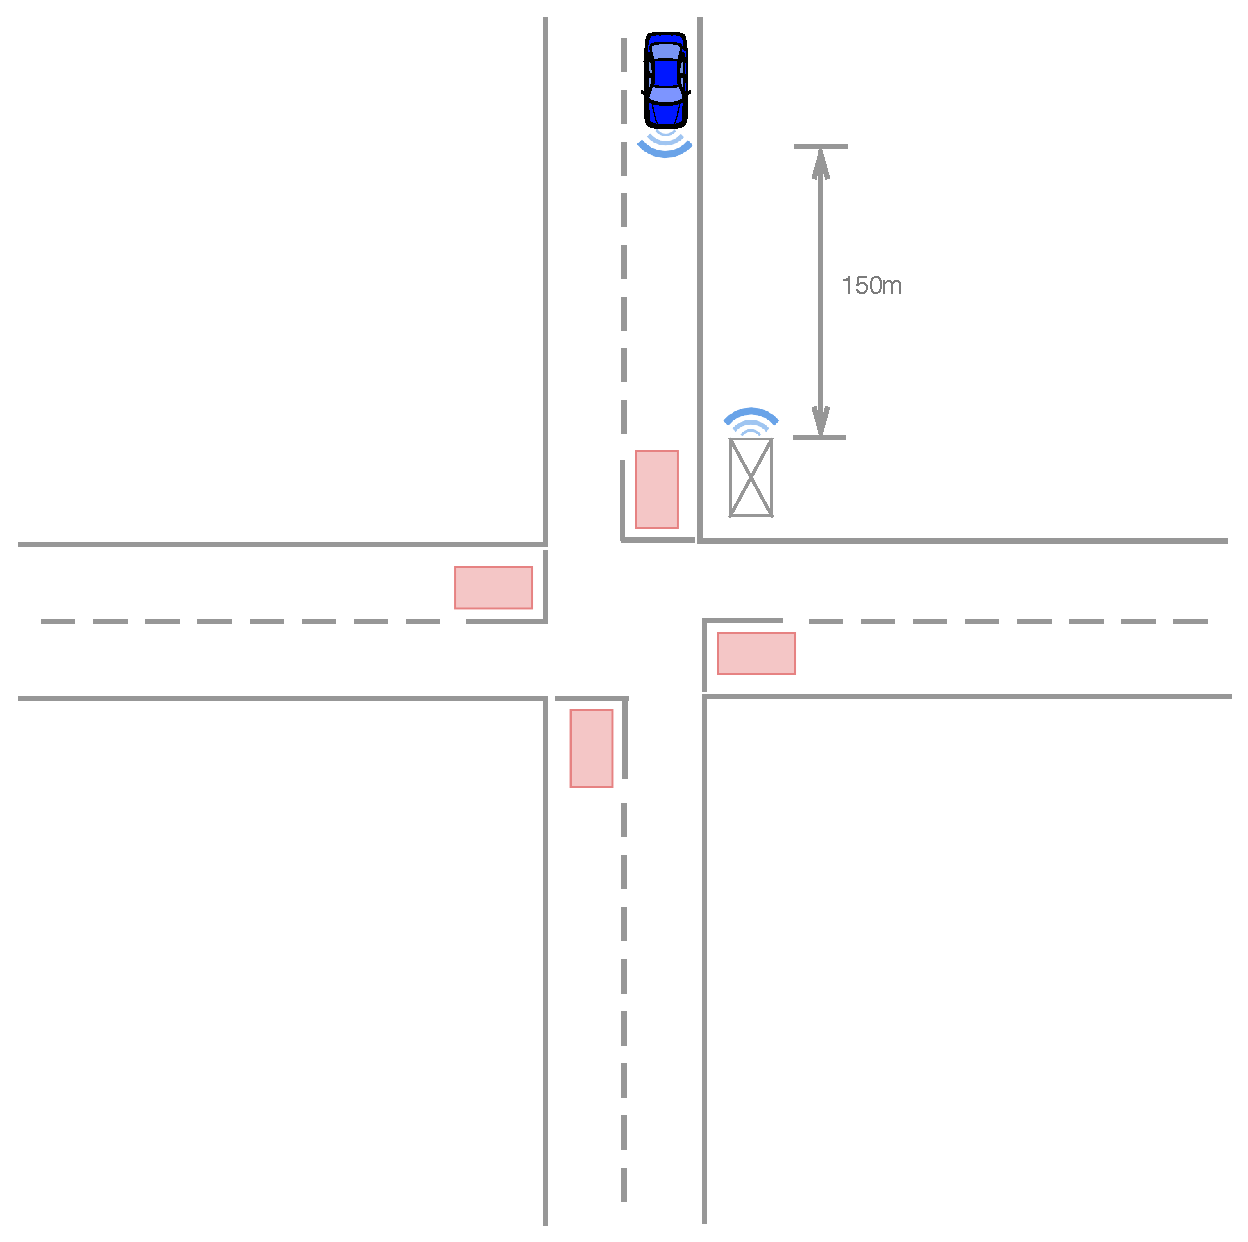
\includegraphics[scale=0.5]{intersection_diagram.eps}
	\caption[Plan of a simple four way intersection showing an approaching vehicle communicating with a traffic controller.]{ Plan of a simple four way intersection showing an approaching vehicle communicating with a PBTC controller. The distance of initial communication is shown as 150 metres. The position of stop-line detectors typically used by SCATS systems are shown in red. The PBTC controller is able to adapt to vehicle actuations in advance of the vehicle's arrival at the stop line. }
\label{intersectiondiagram}
\end{figure}

\subsection {Control Algorithm Design}
\label{sec:PBTCDesign}

The PBTC control algorithm is a primary component of the PBTC system, designed to be executed by a roadside traffic controller to determine which phases should operate, the order of operation, and duration of each phase; in real-time. The primary objective of the PBTC control algorithm is to reduce the total economic cost incurred by vehicle movements  at a PBTC controlled intersection, using traffic composition information communicated to a controller by vehicles in the network. The PBTC control algorithm is similar to the rolling-horizon minimisation algorithm described in more detail in Section \ref{bg:rolling-horizon}. Appendix \ref{appendix:pbtc_algorithm} includes pseudocode of the PBTC control algorithm.

Each intersection phase within the PBTC system contains an allocation of green or red signals to each light at a controlled intersection, such that no two competing traffic flows receive a green light at the same time in a phase. Two traffic flows are said to be competing if a collision would occur if vehicles on each flow entered the intersection at the same time. Each phase also defines a minimum time the phase must run for.  The minimum time condition is a safety consideration of the system, designed to allow enough time for at least one vehicle to pass safely through the intersection before the phase is changed. 

The order and duration of phases at a PBTC controlled intersection is determined by calculating aggregate costs of delay and operation for each approach of an intersection. A PBTC controller maintains a list of messages received from approaching or delayed vehicles that are used for calculation of the delay costs and operational stopping costs for each vehicle and aggregated to find the total costs for an approach. The primary cost of changing phases at a controlled intersection is the cost of stopping and delaying free flowing traffic. As a result, the standard operation for a PBTC controlled intersection is to run a set phase continuously until a phase change is determined to be cost effective and scheduled by the PBTC control algorithm. This behaviour is designed to produce minimal changes to the system, effectively maximising the homogeneity of free flowing traffic until the cost of interfering becomes low relative to the cost of doing nothing. 

A phase change is scheduled by a PBTC controller if the sum of the cost of stopping the traffic flow currently approaching a green signal, defined as the phase change cost or $c_\text{pc}$, is less than the total incurred cost of delay for all vehicles queued and waiting at any approaches displaying a red signal, defined as the phase delay cost or $c_\text{pd}$. The cost of stopping the traffic flow on a green signal also includes an estimation of the potential delay cost for each vehicle assuming they must be delayed \emph{at least} as long as the minimum condition for the newly scheduled phase. Equations \ref{phaseChangeCostEq} and \ref{phaseDelayCostEq} define the phase change cost and phase delay cost. 

\begin{equation}
	c_\text{pc} &= \sum_{v \in A_\text{g}} c_\text{s}(v) + c_{\text{d}(min)}}(v)
	\label{phaseChangeCostEq}
\end{equation}

\begin{equation}
	c_\text{pd} &= \sum_{v \in A_\text{r}} c_\text{d}(v)
	\label{phaseDelayCostEq}
\end{equation}

Where $A_\text{g}$ denotes the set of vehicles approaching a green signal at the intersection, $A_\text{r}$ denotes the set of vehicles approaching or waiting at a red signal at the intersection, $c_\text{s}(v)$ is the incurred cost to a vehicle, $v$ if it is forced to stop, $c_{\text{d}(min)}(v)$ is the incurred cost of delay to vehicle $v$ for as many seconds as the minimum duration of the next phase, and $c_\text{d}(v)$ is the delay cost already incurred by $v$ due to waiting at a red signal. 

The phase change condition is defined by $T = c_\text{pc} - c_\text{d}$. If $T \leq 0$, the algorithm enters a phase change sequence, and a lookahead heuristic is applied to find the minimum potential cost incurred as a result of the change. Based on a predefined lookahead table size, the controller estimates the total cost of changing phase for each second from zero up to the table size, constructing a table with each row representing a time in seconds and the cost of stopping the phase at that time. The controller then dynamically extends the current phase duration by the number of seconds that corresponds with the lowest cost value in the lookahead table. 

The lookahead procedure of the PBTC control algorithm will evaluate the total cost of extending the current phase by a fixed number of seconds to allow the moving vehicles to pass, and extend the current phase by the calculated minimum time if it is found to be less than the cost of an immediate change. For example, if two vehicles are approaching an intersection on a freely flowing approach but are not close enough to the stop-line to pass if the phase is changed immediately, the cost of the change includes the cost of stopping and delaying the the two vehicles for the minimum duration of the next phase. Due to their distance from the intersection and current velocity, after one additional second the two moving vehicles may pass through the intersection and these costs are avoided, with the trade-off cost being one more second of delay for any other vehicles waiting at the intersection. Depending on the delay cost of waiting vehicles, extending the current phase may be preferable. 




